% METODOLOGIA------------------------------------------------------------------

\chapter{DESENVOLVIMENTO DA PESQUISA}
\label{chap:metodologia}


\section{DELINEAMENTO DA PESQUISA}
\label{sec:titSecDelPesq}

Inserir seu texto aqui...

\section{REENGENHARIA DO APLICATIVO MIP/MID}
\label{sec:titSecColDad}
A primeira etapa para a reengenharia no aplicativo foi eu ter que desenvolver as funções lambda para as operações da aplicação. A linguagem que eu adotei para utilização do desenvolvimento das funções Lambda foi Java, pelo fato de ser a mesma linguagem da aplicação original e poder reaproveitar o código e não dificultar manutenção futura. Mas isso foi um grande desafio, pois, pelo fato da aplicação MIP/MID ter sido desenvolvida com o \textit{framework Spring} a aplicação realiza várias configurações por de baixo do pano automaticamente, e quando eu tento replicar essas configurações manualmente não é tão simples quanto parece.

A primeira etapa de desenvolvimento foi encontrar um código de exemplo que estivesse integrando com o AWS Lambda e tenha sido desenvolvido com Java e Hibernate. Felizmente, eu encontrei um código aberto no Github \cite{githubExample}. O exemplo mostra uma implementação simples do Hibernate consumindo as credenciais de acesso via variáveis de ambiente, que será fornecida pela AWS Lambda Function, junto com as depedênicas maven necessárias para se integrar com o serviço AWS. Eu clonei esse projeto do repositório Github e comecei as alterações. A primeira alteração que eu achei útil foi adicionar a dependência \textit{com.amazonaws:aws-lambda-java-events} que permite diferente tipos de entrada para os serviços que invocam a função Lambda, isso se mostrou útil pelo fato de que na função original do exemplo se utilizava de \textit{BufferedReader} para realizar a leitura do corpo da requisição através de binários, o que torna toda leitura e interpretação mais complexa. Com a dependência \textit{aws-lambda-java-events} foi possível capturar o JSON do objeto de uma maneira mais direta, utilizando a classe \textit{APIGatewayProxyRequestEvent} como corpo referente ao request da chamada, e da mesma forma, a biblioteca também facilita gerar uma resposta JSON para o evento utilizando a classe \textit{APIGatewayProxyResponseEvent}.

Com a aplicação de exemplo pronta para ser codificada, eu comecei a trazer as entidades de banco mapeadas com Hibernate para o código. As entidades cujo desenvolvimento eu iniciei foram os da camada Base. Copiei todas as classes e colei dentro de um pacote do projeto Lambda, e a primeira função que eu optei para desenvolver foi de encontrar todos os registros daquela entidade no banco de dados, que pode ser chamado de Get All ou Find All.
\clearpage
\begin{figure}[!htb]
	\centering
	\caption{Código da função GetFields}
	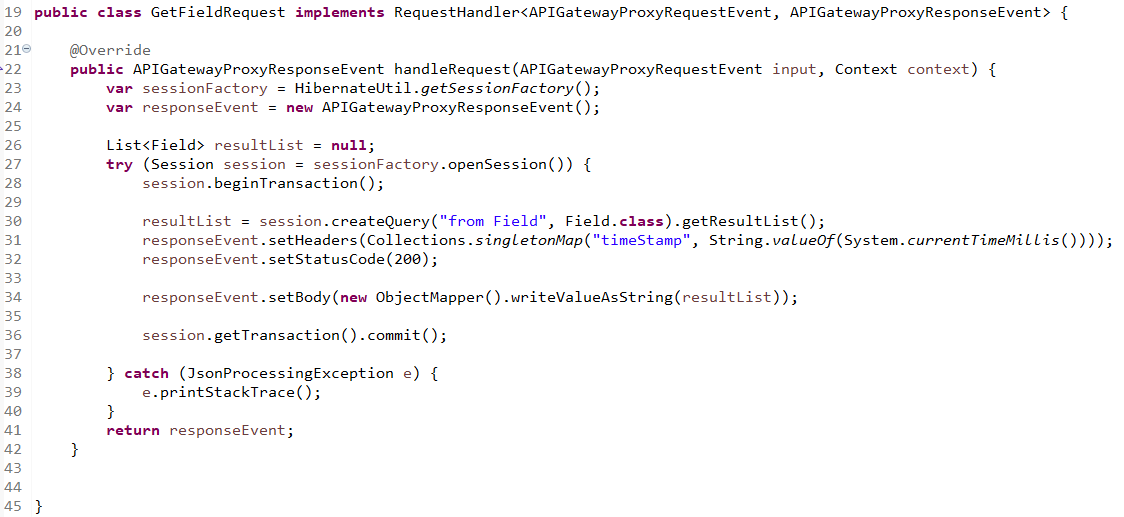
\includegraphics[width=1\textwidth,height=0.4\textheight]{./dados/figuras/codigo-get-fields}
	\fonte{Minha autoria}
	\label{fig:codigo-get-fields}
\end{figure}

A implementação da função para busca de todos elementos da entidade Field pode ser visualizada na Figura \ref{fig:codigo-get-fields}. As primeira coisas a se notar no código são as classes de entrada e saída do \textit{RequestHandler} na linha 19, que são as classes da biblioteca que foi mencionada anteriormente para facilitar a transição de dados da função na plataforma da AWS. A interface obriga a implementação do método \textit{handleRequest}: esse método será acionado quando for parametrizado na função. Perceba pela sintaxe da linha 23 e 24 que está utilizando a tipagem \textit{var}, com isso podemos inferir que código roda somente no JDK 10 para cima, no lambda permite-se o código Java 8 e 11 somente, que são as versões LTS atuais, e como o código original foi escrito em Java 11, as funções Lambda também serão escritas da mesma forma. Na linha 23 eu instancio uma sessão hibernate através da classe útil fornecida pelo exemplo e inicio a conexão com o banco na linha 27 com o recurso \textit{try-catch-with-resources}, que fechará a conexão automaticamente após o fechamento do bloco. No começo do bloco dou inicio a uma transação e realizo uma chamada no banco de dados na linha para buscar todos os resultados possíveis que estão registrados na tabela Field. Desta forma, o resultado  do banco é armazenado na variável resultList, e começo montando o objeto de resposta setando o cabeçalho e o status code da chamada. Esse response será disponibilizado para o API Gateway poder retornar essa mesma informação. Na linha 34 eu seto o corpo da resposta, serializando o objeto Java em um JSON String para que possa ser disponibilizado como recurso consumível no API Gateway e por fim na filha 36 eu commito a transação e retorno na linha 41.

Com o código da primeira função finalizada, eu acesso a plataforma da AWS e eu vou primeiramente criar uma rota no serviço API Gateway para servir de gatilho para minha função. Após a API criada, o próximo passo é criar um recurso chamado /field e um sub-recurso chamado /all, dentro desses recursos eu cadastro os métodos HTTPs que serão utilizado dentro deles. Para a busca de todos os elementos e tentar respeitar os níveis de maturidade do modelo de Richardson para API REST, eu crio um metódo GET dentro do sub-recurso all e realizo o deploy da API para disponibilizar em um endpoint público.

\begin{figure}[!htb]
	\centering
	\caption{API Gateway}
	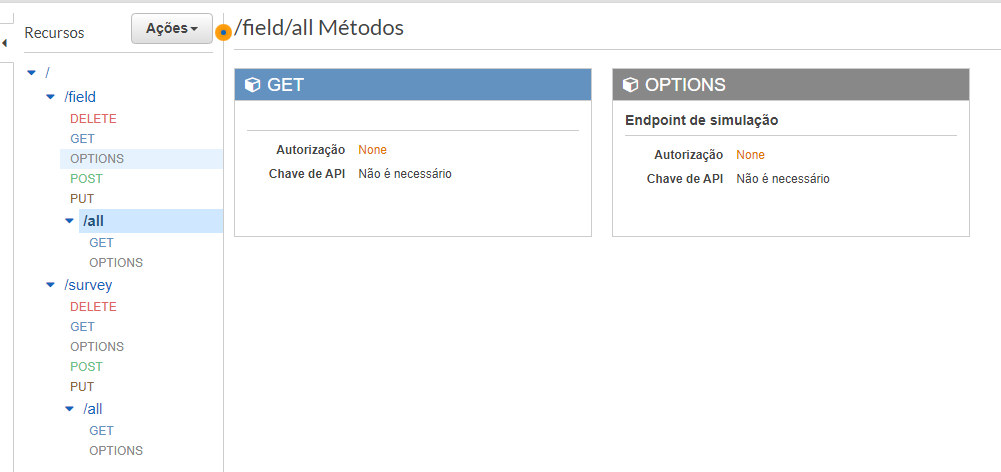
\includegraphics[width=1\textwidth,height=0.4\textheight]{./dados/figuras/api-gateway}
	\fonte{Minha autoria}
	\label{fig:api-gateway}
\end{figure}

No próximo passo, eu crio uma função Lambda na plataforma da AWS e realizo o upload do JAR executável da aplicação, e aplico o caminho da função dentro do JAR para que a plataforma consiga encontrar o método \textit{handleRequest} que foi implementado.

\begin{figure}[!htb]
	\centering
	\caption{Função Lambda para buscar todos Fields}
	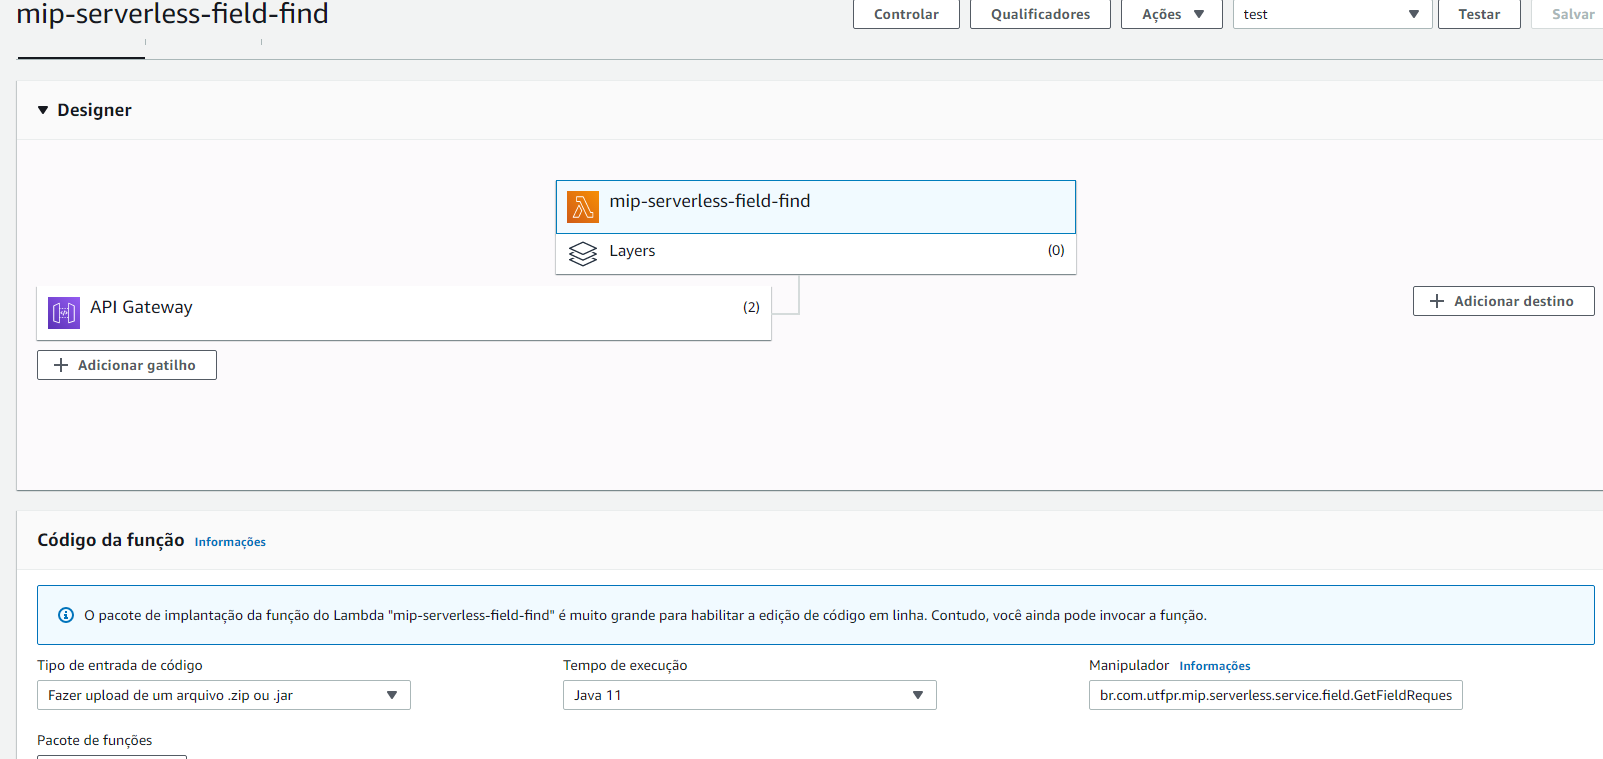
\includegraphics[width=1\textwidth,height=0.5\textheight]{./dados/figuras/lambda-field-get}
	\fonte{Minha autoria}
	\label{fig:lambda-field-get}
\end{figure}

\begin{figure}[!htb]
	\centering
	\caption{Variáveis de ambiente para se conectar no RDS}
	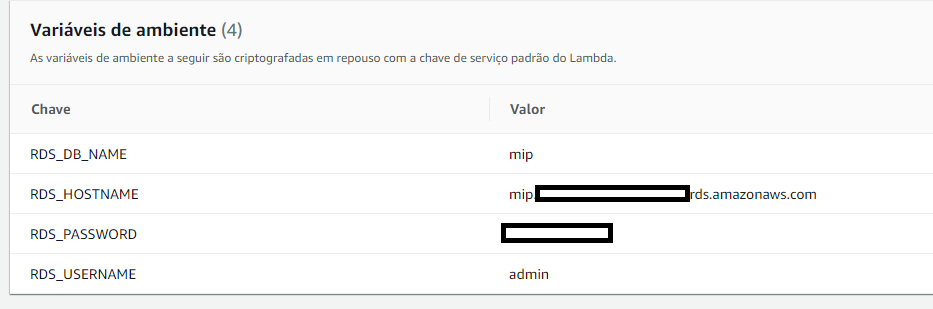
\includegraphics[width=1\textwidth,height=0.2\textheight]{./dados/figuras/credenciais-lambda}
	\fonte{Minha autoria}
	\label{fig:credenciais-lambda}
\end{figure}

Na figura \ref{fig:lambda-field-get} eu mostro como fica na plataforma AWS a função já configurada. O serviço precisa ser ativado através de algum caminho, e é possível configurar esse gatilho no campo designer, conforme a figura, sendo que nesse campo eu consigo apontar qual recurso REST configurado no API Gateway, que eu já criei, eu quero que acione minha função lambda. Na figura \ref{fig:credenciais-lambda} eu mostro como fica o campo de varáveis de ambiente após ter sido devidamente preenchida para que seja possível a aplicação se conectar com o banco.

\begin{figure}[!htb]
	\centering
	\caption{Teste de chamada da função lambda}
	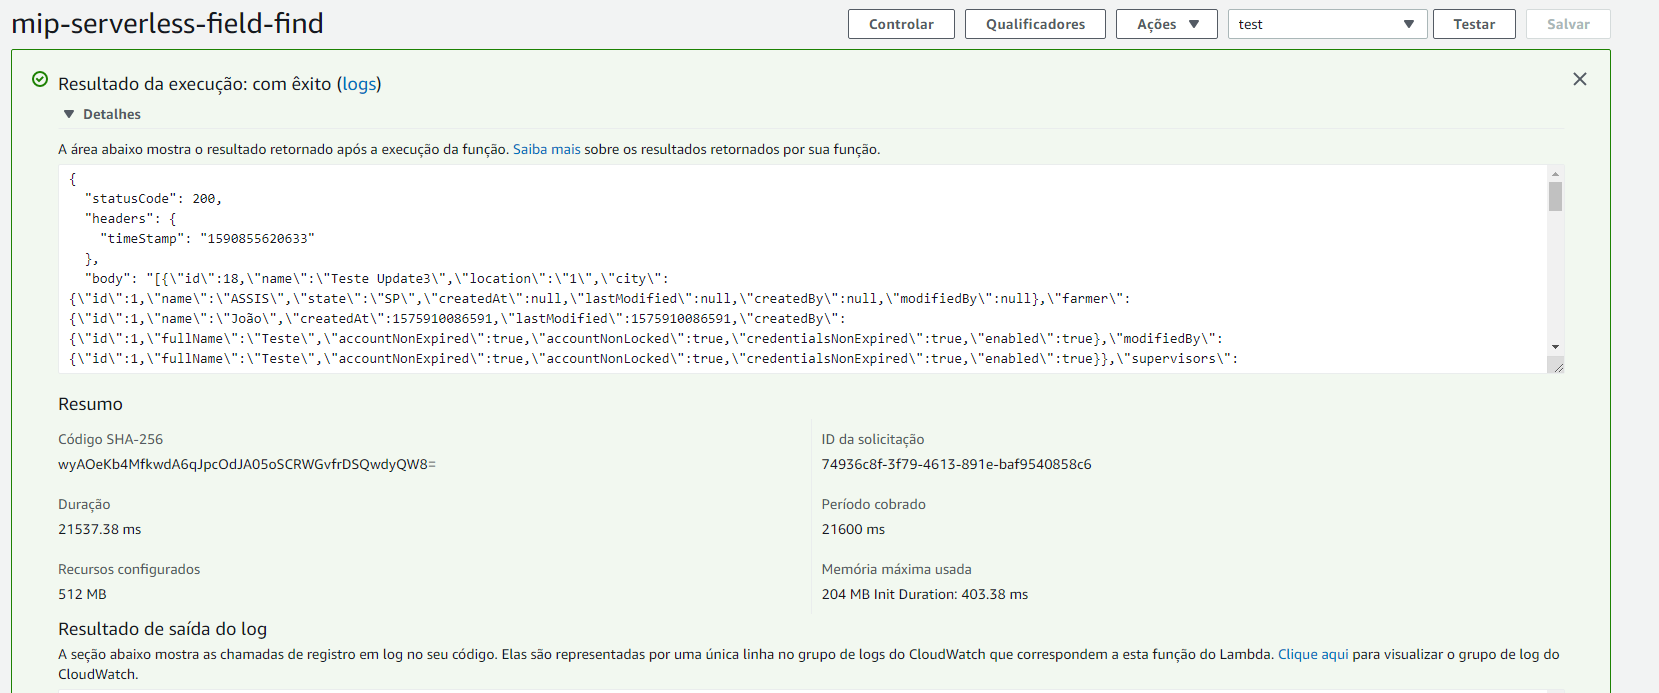
\includegraphics[width=1\textwidth,height=0.3\textheight]{./dados/figuras/lambda-test}
	\fonte{Minha autoria}
	\label{fig:lambda-test}
\end{figure}

Com todos os parâmetros configurados, eu posso realizar um teste de chamada da função conforme eu mostro na figura \ref{fig:lambda-test}, eu consigo montar um corpo em JSON para simular uma chamada REST, mas como essa função em especifico não possui parâmetros e retorna todos os elementos do banco basta clicar no botão teste para visualizar o resultado. E conforme mostra na figura acima é possível visualizar o JSON mostrando informações das entidades cadastradas.

Com o IP público da API REST disponibilizado, eu vou até a aplicação original do MIP/MID e cadastro como propriedade a respectiva URL, no arquivo \texttt{application.properties}. Após isso crio um novo pacote nomeado de Lambda no projeto e a classe \texttt{FieldLambda} para fazer o papel de wrapper de todas as chamadas Lambda referente a camada Field. Para facilitar as chamadas REST eu adicionei a dependência do Unirest, que é uma biblioteca em java para abstrair e facilitar requisições para APIs. Na imagem \ref{fig:field-lambda-service} eu mostro como fica a implementação para acionar a função lambda na AWS, na linha 29 e 30 eu busco a URL pública e armazeno na variável \texttt{ENDPOINT\_GATEWAY} e crio o método readAll, utilizando a biblioteca Unirest para realizar a chamada GET na API.

\begin{figure}[!htb]
	\centering
	\caption{Serviço para acionar função Lambda}
	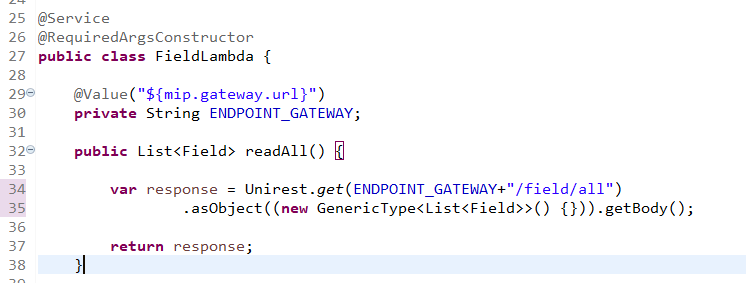
\includegraphics[width=1\textwidth,height=0.3\textheight]{./dados/figuras/field-lambda-service}
	\fonte{Minha autoria}
	\label{fig:field-lambda-service}
\end{figure}

\clearpage
Com a estrutura criada para acionar a função Lambda, eu vou até o a camada de serviço e procuro pelo classe responsável por Field e pelo método readAll, que faz consulta direto no banco e simplesmente deleto o método, após isso vejo na aplicação inteira onde o código quebrou por conta da falta do método, e vou um a um substituindo pela nova chamada Lambda. Feito isso, a aplicação agora está se integrando com o Lambda da AWS chamando a função para buscar todos os Fields.

Para os outros cenários se manteve exatamente a mesma estratégia, diferindo somente nas regras de negócios mais especificas, tais como, validações de inserção e atualização de dados, permissão para deleção, mas tudo isso ficou contido dentro da função Lambda. E as novas funções ficaram continuas em um só projeto Java, e quando feito o upload do JAR é especificado o caminho especifico do \textit{handler} daquela função dentro do projeto.